\part{Spring Basics}


\begin{frame}{Spring Ecosystem}
	\begin{figure}
  	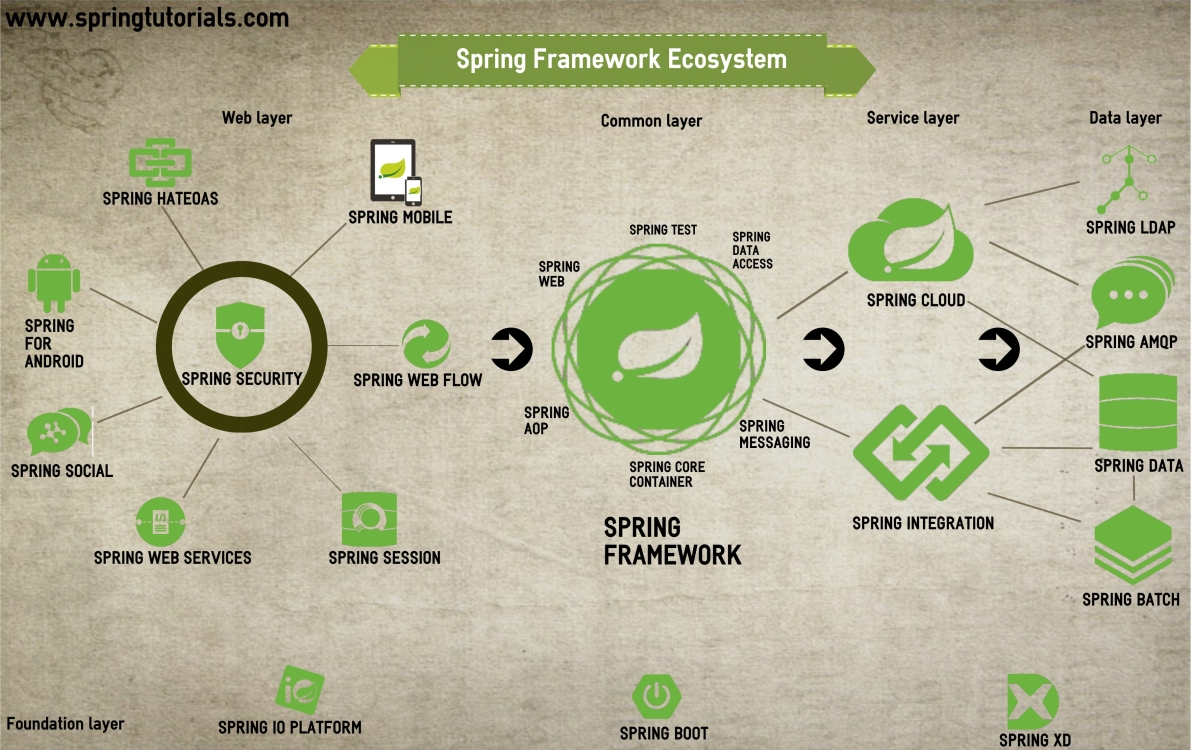
\includegraphics[height=0.7\textheight]{../SpringBasics/images/spring-ecosystem}
	\end{figure}
 \colorlink{http://spring.io/}{http://spring.io/}
\end{frame}

\begin{frame}[fragile]{What is wrong with this picture?}
\begin{figure}
	\includeExplainIoC{width=0.9\textwidth}
\end{figure}
How easy is it to replace the implementation of  \textit{\codealt{CreditCheck}}
\begin{itemize}
	\item during runtime
	\item when referenced by multiple other objects
	\item with a Mock within an Integration Test?
\end{itemize}
\end{frame}

\begin{frame}{Dependency Injection with Spring}
\begin{block}{\emph{Spring Core} offers a Dependency Injection framework}
\begin{itemize}
\item one form of Inversion of Control (IoC)
\item separates definition from creation from usage
\item eases the replacement of dependencies during runtime\\(especially relevant in context of tests)
\end{itemize}
\end{block}
\vfill
\begin{visibleenv}<2->
That means \ldots
\begin{itemize}
\item YOU define which objects are created how
	\begin{itemize}
	\item Spring creates/manages objects in application context
	\end{itemize}
\item YOU define dependencies
	\begin{itemize}
	\item Spring injects required dependencies
	\end{itemize}
\end{itemize}
\end{visibleenv}
\end{frame}


\begin{frame}[fragile]{Classic: Direct Instantiation}
\begin{figure}
\includeGraphicsNoSpring{height=0.7\textheight}
\end{figure}
\end{frame}

\begin{frame}[fragile]{Dependency Injection by Spring}
\begin{figure}
\includeGraphicsSpring{height=0.7\textheight}
\end{figure}
\end{frame}

\begin{frame}[fragile]{Dependency Injection for Testing}
\begin{figure}
\includeGraphicsSpringInTest{height=0.7\textheight}
\end{figure}
\end{frame}


\begin{frame}[fragile]{Setup Spring Application Context - Explicitly}
Ways of defining \textbf{\emph{Beans}} - classes managed by Spring:
\begin{itemize}
	\item XML-based i.e. \codealt{WEB-INF/web.xml}
	\item Java Code-based (preferred)
\end{itemize}
\vfill
\begin{visibleenv}<2>
\begin{block}{Example: Explicit registration}
\begin{lstlisting}[language=Java]
AnnotationConfigWebApplicationContext context = new AnnotationConfigWebApplicationContext();

context.register(CreditCheckImpl.class);
context.register(WebShop.class);
...
context.refresh(); // completes Bean registration
\end{lstlisting}
\vspace{-5mm}	
\end{block}
\end{visibleenv}
\end{frame}


\begin{frame}[fragile]{Setup Spring Application Context - Implicitly}
Define discoverable \textbf{\emph{Beans}} in \textbf{\codealt{@Component}} and \textbf{\codealt{@Configuration}} annotated classes
\begin{columns}
\begin{column}[T]{.47\textwidth}
\begin{visibleenv}<2->
\begin{block}{Example: @Component}
\begin{lstlisting}[language=Java]
// defines Bean with id "creditCheck"
@Component("creditCheck") 
public class CreditCheckImpl implements CreditCheck {
   ...
}
\end{lstlisting}	
\end{block}
\end{visibleenv}
\end{column}
\begin{column}[T]{.47\textwidth}
\begin{visibleenv}<3->
\begin{block}{Example: @Configuration}
\begin{lstlisting}[language=Java,belowskip=0mm,aboveskip=0mm]
// includes scan of sub packages
@ComponentScan("com.sap.mypackage") 
// source of Bean definitions
@Configuration
public class AppContextConfig {
	
   @Bean //defines "myWebShop" Bean
   public WebShop myWebShop() {
      return new WebShop();
   }
}
\end{lstlisting}
\end{block}
\end{visibleenv}
\end{column}
\end{columns}
\begin{visibleenv}<4>
\begin{itemize}
     \item \textbf{\codealt{@ComponentScan}} defines search scope for \emph{Beans}
	\item Explicitly register \codealt{AppContextConfig} as root config class
\end{itemize}
\end{visibleenv}
\end{frame}

\begin{frame}[fragile]{Define Dependencies to be Injected}
Define dependent \textbf{\emph{Beans}}\footnote{Never instantiate \emph{Beans} using the \codealt{new} keyword!} to be injected
\begin{itemize}
	\item Constructor Injection (for defining required dependencies)
	\item Setter Injection (for optional and configurable values)
	\item Field Injection (not recommended)
\end{itemize}
\vfill
\begin{visibleenv}<2>
\begin{block}{Example: Constructor Injection}
\begin{lstlisting}[language=Java,belowskip=0mm,aboveskip=0mm]
public class WebShop { // Note: WebShop needs to be a Spring managed class!

    private final CreditCheck creditCheck;
	
    @Inject // or @Autowired
    public WebShop(CreditCheck creditCheck) { // arguments provided by Spring
        this.creditCheck = creditCheck;
    }
}
\end{lstlisting}
\vspace{-5mm}	
\end{block}
\end{visibleenv}
\end{frame}

\begin{frame}[fragile]{Scoping Beans - Define Object Lifecycle}
\begin{description}
\item[\underline{Singleton}] default: object is created once for entire application\newline => for stateless objects only
\item[Prototype] object is created when injected
\item[Request] in a web application, object is created for each request
\item[Session] in a web application, object is created for each session
\end{description}
\vfill
\begin{block}{Example: Define request scoped \emph{Bean}}
\begin{lstlisting}[language=Java,belowskip=0mm,aboveskip=0mm]
@Bean // or @Component or @Configuration ...
@Scope(ConfigurableBeanFactory.SCOPE_REQUEST)
\end{lstlisting}
\vspace{-5mm}	
\end{block}
\end{frame}

\begin{frame}[fragile]{Environments and Profiles}
Examples for environments: development, test, cloud (production)
\begin{itemize}
\item The Environment is defined with \textit{Active Profiles}, e.g.:
\begin{lstlisting}
applicationContext.getEnvironment().setActiveProfiles("cloud");
\end{lstlisting}
\item \codealt{@Profile} defines environment specific \emph{Bean}, ensures that \emph{Bean} is only registered when "cloud" profile is active
\begin{lstlisting}
@Bean // or @Component or @Configuration ...
@Profile("cloud")
\end{lstlisting}
\end{itemize}
\vfill
\begin{visibleenv}<2>
Annotations for managing ambiguous \emph{Beans} of the same type:
\begin{itemize}
\item \codealt{@Primary} designates a primary \emph{Bean}
\item \codealt{@Qualifier("beanId")} chooses an unique \emph{Bean} for injection
\end{itemize}
\end{visibleenv}
\end{frame}

\begin{frame}{Further Reading}
\textbf{References}
\begin{itemize}
\item \colorlink{http://docs.spring.io/spring-framework/docs/current/javadoc-api/org/springframework/context/annotation/Configuration.html}{Java Doc: @Configuration}
\item \colorlink{https://github.wdf.sap.corp/d022051/SpringTutorial/wiki/SpringContext}{SAP: Spring Context explained}
\item \colorlink{https://spring.io/blog/2007/07/11/setter-injection-versus-constructor-injection-and-the-use-of-required/}{Blog: Setter injection versus constructor injection}
\item \colorlink{http://docs.spring.io/spring/docs/current/spring-framework-reference/html/index.html}{Spring Framework Reference}
\end{itemize}
\vfill
\textbf{Recommended Books}\newline\newline
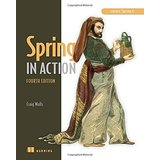
\includegraphics[height=22mm]{../SpringBasics/images/SpringInAction}  

\includegraphics[height=22mm]{../SpringBoot/images/SpringBootInAction}
\end{frame}
